% Options for packages loaded elsewhere
\PassOptionsToPackage{unicode}{hyperref}
\PassOptionsToPackage{hyphens}{url}
\PassOptionsToPackage{dvipsnames,svgnames,x11names}{xcolor}
\documentclass[
  10pt,
  fontset=fandol]{ctexart}
\usepackage{xcolor}
\usepackage[margin=16mm]{geometry}
\usepackage{amsmath,amssymb}
\setcounter{secnumdepth}{-\maxdimen} % remove section numbering
\usepackage{iftex}
\ifPDFTeX
  \usepackage[T1]{fontenc}
  \usepackage[utf8]{inputenc}
  \usepackage{textcomp} % provide euro and other symbols
\else % if luatex or xetex
  \usepackage{unicode-math} % this also loads fontspec
  \defaultfontfeatures{Scale=MatchLowercase}
  \defaultfontfeatures[\rmfamily]{Ligatures=TeX,Scale=1}
\fi
\usepackage{lmodern}
\ifPDFTeX\else
  % xetex/luatex font selection
\fi
% Use upquote if available, for straight quotes in verbatim environments
\IfFileExists{upquote.sty}{\usepackage{upquote}}{}
\IfFileExists{microtype.sty}{% use microtype if available
  \usepackage[]{microtype}
  \UseMicrotypeSet[protrusion]{basicmath} % disable protrusion for tt fonts
}{}
\makeatletter
\@ifundefined{KOMAClassName}{% if non-KOMA class
  \IfFileExists{parskip.sty}{%
    \usepackage{parskip}
  }{% else
    \setlength{\parindent}{0pt}
    \setlength{\parskip}{6pt plus 2pt minus 1pt}}
}{% if KOMA class
  \KOMAoptions{parskip=half}}
\makeatother
\usepackage{longtable,booktabs,array}
\newcounter{none} % for unnumbered tables
\usepackage{calc} % for calculating minipage widths
% Correct order of tables after \paragraph or \subparagraph
\usepackage{etoolbox}
\makeatletter
\patchcmd\longtable{\par}{\if@noskipsec\mbox{}\fi\par}{}{}
\makeatother
% Allow footnotes in longtable head/foot
\IfFileExists{footnotehyper.sty}{\usepackage{footnotehyper}}{\usepackage{footnote}}
\makesavenoteenv{longtable}
\usepackage{graphicx}
\makeatletter
\newsavebox\pandoc@box
\newcommand*\pandocbounded[1]{% scales image to fit in text height/width
  \sbox\pandoc@box{#1}%
  \Gscale@div\@tempa{\textheight}{\dimexpr\ht\pandoc@box+\dp\pandoc@box\relax}%
  \Gscale@div\@tempb{\linewidth}{\wd\pandoc@box}%
  \ifdim\@tempb\p@<\@tempa\p@\let\@tempa\@tempb\fi% select the smaller of both
  \ifdim\@tempa\p@<\p@\scalebox{\@tempa}{\usebox\pandoc@box}%
  \else\usebox{\pandoc@box}%
  \fi%
}
% Set default figure placement to htbp
\def\fps@figure{htbp}
\makeatother
\setlength{\emergencystretch}{3em} % prevent overfull lines
\providecommand{\tightlist}{%
  \setlength{\itemsep}{0pt}\setlength{\parskip}{0pt}}
\usepackage{amsmath,amssymb,mathtools,needspace}
\xeCJKDeclareCharClass{CJK}{"2032,"0400->"04FF,"2160->"216B,"2460->"2473,"25A0,"25C7,"25CB,"25CF}
\IfFontExistsTF{Arial Unicode MS}{\xeCJKsetup{AutoFallBack=true}\setCJKfallbackfamilyfont{\CJKrmdefault}{Arial Unicode MS}}{}
\setcounter{secnumdepth}{0}
\setlength{\emergencystretch}{2em}
\allowdisplaybreaks
\usepackage{bookmark}
\IfFileExists{xurl.sty}{\usepackage{xurl}}{} % add URL line breaks if available
\urlstyle{same}
\hypersetup{
  pdftitle={中点方法},
  colorlinks=true,
  linkcolor={Maroon},
  filecolor={Maroon},
  citecolor={Blue},
  urlcolor={Blue},
  pdfcreator={LaTeX via pandoc}}

\title{中点方法}
\author{}
\date{}

\begin{document}
\maketitle

\subsubsection{4.5.1 中点方法}\label{ux4e2dux70b9ux65b9ux6cd5}

按照数学分析的定义，导数 \(f'(a)\) 是差商 \(\dfrac{f(a+h)-f(a)}h\) 当 \(h\to0\) 时的极限。如果精度要求不高，我们可以简单地取差商作为导数的近似值，这样便建立起一种数值微分方法，即

\[
f'(a)\approx\frac{f(a+h)-f(a)}h.
\]

类似地，亦可用向后差商作近似运算，即

\[
f'(a)\approx\frac{f(a)-f(a-h)}h
\]

或用中心差商作近似计算，即

\[
f'(a)\approx\frac{f(a+h)-f(a-h)}{2h}.
\]

后一种数值微分方法称中点方法，它其实是前两种方法的算术平均。

在图 4.3 上，上述三种导数的近似值分别表示弦线 \(AB\)、\(AC\) 和 \(BC\) 的斜率，比较这三种弦线与切线 \(AT\)（其斜率等于导数值 \(f'(a)\)）平行的程度，从图形上可以明显地看出，其中以 \(BC\) 的斜率更接近于切线 \(AT\) 的斜率。因此就精度而言，以中点方法更为可取。

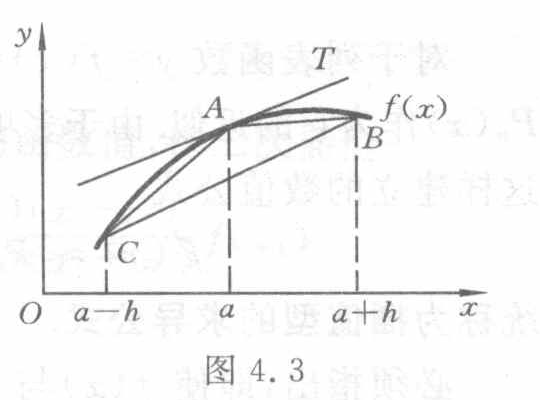
\includegraphics[width=0.85\linewidth,height=\textheight,keepaspectratio,alt={图 4.3（原书扫描裁切）}]{../assets/ch04b/figure-4-3.png}

图 4.3。原图标签：横轴 \(x\)、纵轴 \(y\)、原点 \(O\)；横轴位置 \(a-h\)、\(a\)、\(a+h\)，对应曲线上的点 \(C\)、\(A\)、\(B\)；曲线标记 \(f(x)\)，过 \(A\) 的切线标记 \(T\)。图中画出弦线 \(AB\)、\(AC\)、\(BC\) 与切线 \(AT\)。（此段为图中标签和图意的文字转录；原图未给出具体函数或数值。）

上述三种数值微分方法有个共同点，它们都是将导数的计算归结为计算 \(f\) 在若干节点上的函数值。这类数值微分方法称为机械求导方法。

要利用中点公式

\[
G(h)=\frac{f(a+h)-f(a-h)}{2h}
\]

计算导数 \(f'(a)\) 的近似值，首先必须选取合适的步长，为此需要进行误差分析。分别将 \(f(a\pm h)\) 在 \(x=a\) 处作 Taylor 展开，有

\[
f(a\pm h)=f(a)\pm hf'(a)+\frac{h^2}{2!}f''(a)
\pm\frac{h^3}{3!}f'''(a)+\frac{h^4}{4!}f^{(4)}(a)
\pm\frac{h^5}{5!}f^{(5)}(a)+\cdots,
\]

代入上式得

\[
G(h)=f'(a)+\frac{h^2}{3!}f'''(a)+\frac{h^4}{5!}f^{(5)}(a)+\cdots.
\]

\href{../../source-images/pdf-113.jpeg}{原页图像}

\subsubsection{4.5.1 中点方法（续）}\label{ux4e2dux70b9ux65b9ux6cd5ux7eed}

由此得知，从截断误差的角度看，步长越小，计算结果越准确。

再考察舍入误差，按中点公式计算。当 \(h\) 很小时，因 \(f(a+h)\) 与 \(f(a-h)\) 很接近，直接相减会造成有效数字的严重损失（参见 1.4 节）。因此，从舍入误差的角度来看，步长是不宜太小的。

例如，用中点公式求 \(f(x)=\sqrt{x}\) 在 \(x=2\) 处的一阶导数，有

\[
G(h)=\frac{\sqrt{2+h}-\sqrt{2-h}}{2h}.
\]

设取四位数字计算，结果如表 4.6（导数的准确值 \(f'(2)=0.353\,553\)）所示。

\textbf{表 4.6}

{\def\LTcaptype{none} % do not increment counter
\begin{longtable}[]{@{}rrrrrr@{}}
\toprule\noalign{}
\(h\) & \(G(h)\) & \(h\) & \(G(h)\) & \(h\) & \(G(h)\) \\
\midrule\noalign{}
\endhead
\bottomrule\noalign{}
\endlastfoot
\(1\) & \(0.366\,0\) & \(0.05\) & \(0.353\,0\) & \(0.001\) & \(0.350\,0\) \\
\(0.5\) & \(0.356\,4\) & \(0.01\) & \(0.350\,0\) & \(0.000\,5\) & \(0.300\,0\) \\
\(0.1\) & \(0.353\,5\) & \(0.005\) & \(0.350\,0\) & \(0.000\,1\) & \(0.300\,0\) \\
\end{longtable}
}

在表 4.6 中，\(h=0.1\) 的逼近效果最好，如果进一步缩小步长，则逼近的效果会越来越差。

\begin{center}\rule{0.5\linewidth}{0.5pt}\end{center}

\subsection{相关原页校注（agent 补充）}\label{ux76f8ux5173ux539fux9875ux6821ux6ce8agent-ux8865ux5145}

以下校注来自本节覆盖的原页，可能也涉及同页相邻小节；原文照录与校正说明分开保留。

\subsubsection{原书 PDF 页 113 的校注}\label{ux539fux4e66-pdf-ux9875-113-ux7684ux6821ux6ce8}

\href{../pages/pdf-113.md}{完整原页转录} · \href{../../source-images/pdf-113.jpeg}{原页图像}

校注记录：CH04B-E004。

\begin{quote}
校注（agent 补充，CH04B-E004）：原页``其中''后的节点多项式印为 \(\prod_{k=0}^{n}(x-x_i)\)，乘积指标 \(k\) 与因子下标 \(i\) 不一致，已按原扫描保留。结合本页表 4.7 和下文 \(\omega_{n+1}(x_k)=0\)，应将因子写作 \((x-x_k)\)，或统一将乘积指标改为 \(i\)；这是原书疑似下标排印错误，非 OCR 错误。\href{../assets/ch04b/review-p113-product.png}{局部原扫描}。
\end{quote}

\subsection{本节覆盖原页的校注记录}\label{ux672cux8282ux8986ux76d6ux539fux9875ux7684ux6821ux6ce8ux8bb0ux5f55}

下列记录按原页关联，含同页相邻小节的校注；计算时同时读取上文校注和完整原页。

\begin{itemize}
\tightlist
\item
  \texttt{CH04B-E004}：原书 PDF 页 113
\end{itemize}

\end{document}
